\section{Preliminaries}
\label{section_preliminaries}

\subsection{Permutations and ordered partitions}

Let $\Sym_{n}$ denote the symmetric group on $n$ elements.
We write permutations $\tau \in \Sym_{n}$ in one-line notation, that is,
$\tau = \tau_{1} \tau_{2} \cdots \tau_{n}$.
Let the symmetric group $\Sym_{n}$ act upon the
vector space~$\Rrr^{n}$ by permuting the coordinates,
that is,
given a permutation $\tau$
and the vector $x = (x_{1}, x_{2}, \ldots, x_{n})$,
we define
$\tau(x) = (x_{\tau^{-1}(1)}, x_{\tau^{-1}(2)}, \ldots, x_{\tau^{-1}(n)})$.
This is a left action, since
for two permutations $\tau$ and $\pi$ we have that
$\tau(\pi(x)) = (\tau \circ \pi)(x)$.

Define $[n]$ to be the set $\{1,2, \ldots, n\}$.
We will need the following permutation statistics.
The \emph{descent set} of a permutation $\tau \in \Sym_{n}$
is the set
$\Des(\tau) = \{i \in [n-1] \: : \: \tau_{i} > \tau_{i+1}\}$.
The \emph{descent composition} is the list
$(d_{1}-d_{0}, d_{2}-d_{1}, \ldots, d_{k+1}-d_{k})$
where $\Des(\tau) = \{d_{1} < d_{2} < \cdots < d_{k}\}$
and we tacitly assume $d_{0} = 0$ and $d_{k+1} = n$.
The \emph{number of inversions} of a permutation, also called the
\emph{length},
is given by
$\inv(\tau) = |\{(i,j) \: : \: 1 \leq i < j \leq n, \tau_{i} > \tau_{j}\}|$.
Finally, denote the \emph{sign} of a permutation $\tau$ by
$(-1)^{\tau}$, that is,
$(-1)^{\tau} = (-1)^{\inv(\tau)}$.

In the symmetric group $\Sym_{n}$
let $s_{i}$ denote the simple transposition $(i,i+1)$
where $1 \leq i \leq n-1$.
The \emph{weak Bruhat order} on the symmetric group $\Sym_{n}$
is defined by the cover relation
$\tau \coveredby \tau s_{i}$ where
$\inv(\tau) < \inv(\tau s_{i})$.
More explicitly, the cover relation is
$$
\tau_{1} \cdots \tau_{i} \tau_{i+1} \cdots \tau_{n}
\coveredby
\tau_{1} \cdots \tau_{i+1} \tau_{i} \cdots \tau_{n}
\:\:\:\:
\text{ if }
\:\:\:\:
\tau_{i} < \tau_{i+1} .
$$
With respect to this partial order,
the identity element $12 \cdots n$ is the minimal element,
the permutation $n \cdots 21$ is the maximal element,
and the rank function is given by the number of inversions
of the permutation.



The $(n-1)$-dimensional
\emph{permutahedron} 
is the simple polytope defined by
taking the convex hull of the $n!$ points 
$(\tau_{1}, \tau_{2}, \ldots, \tau_{n}) \in \Rrr^{n}$
where $\tau \in \Sym_{n}$.
These $n!$ points lie in the hyperplane
$\sum_{i=1}^{n} x_{i} = \binom{n+1}{2}$,
%$x_{1} + x_{2} + \cdots + x_{n} = 1 + 2 + \cdots + n$,
and one can verify
they generate a
polytope of dimension $n-1$.
Label the vertex
$(\tau_{1}, \tau_{2}, \ldots, \tau_{n})$ by the inverse permutation $\tau^{-1}$.
The $1$-skeleton of the $(n-1)$-dimensional permutahedron
yields the Hasse diagram of the weak Bruhat order of $\Sym_{n}$,
where the cover relations are oriented away from
the vertex labeled $12 \cdots n$ and toward the vertex labeled $n \cdots 21$.




A \emph{partition} $\pi = \{B_{1}, B_{2}, \ldots, B_{k}\}$
of the set $[n]$ is a collection of subsets of~$[n]$, called \emph{blocks},
such that $B_{i} \neq \emptyset$ for $1 \leq i \leq k$,
$B_{i} \cap B_{j} = \emptyset$ for $1 \leq i < j \leq k$
and
$\bigcup_{i=1}^{k} B_{i} = [n]$.
Let $\Pi_{n}$ denote
the collection of all the partitions of the set $[n]$.
We make $\Pi_{n}$ into a partially ordered set (poset)
by the cover relation
$$
  \{B_{1}, B_{2}, B_{3}, \ldots, B_{k}\}
  \coveredby
  \{B_{1} \cup B_{2}, B_{3}, \ldots, B_{k}\} .
$$
In other words, $\Pi_{n}$ is ordered by reverse refinement.
The poset $\Pi_{n}$ is in fact a lattice,
known as the \emph{partition lattice}.
Furthermore, the partition lattice $\Pi_{n}$ is a graded poset,
with minimal element
$\hz = \{\{1\}, \{2\}, \ldots, \{n\}\}$,
maximal element
$\ho = \{[n]\}$
and rank function
$\rho(\pi) = n-|\pi|$,
where
$|\pi|$ denotes the number of blocks of the partition $\pi$.



An \emph{ordered partition} 
$\sigma = (C_{1}, C_{2}, \ldots, C_{k})$
of the set $[n]$
is a list of subsets of $[n]$ such that
$\{C_{1}, C_{2}, \ldots, C_{k}\}$
is a partition of $[n]$.
Let $\Qn$ denote the set of all
ordered partitions on the set~$[n]$.
The set $\Qn$ forms a poset
by letting the cover relation
be the merging of two adjacent blocks, that is,
$$
(C_{1}, \ldots, C_{i}, C_{i+1}, \ldots, C_{k})
\coveredby
(C_{1}, \ldots, C_{i} \cup C_{i+1}, \ldots, C_{k}) .
$$
Observe that the maximal element of
$\Qn$ is
the ordered partition consisting of one block~$([n])$.
However there are $n!$ minimal elements,
one for each permutation $\tau = \tau_{1} \tau_{2} \cdots \tau_{n}$
in the symmetric group $\Sym_{n}$, namely
the ordered partitions of the form
$(\{\tau_{1}\}, \{\tau_{2}\}, \ldots, \{\tau_{n}\})$.
We identify these minimal elements with
permutations in~$\Sym_{n}$ written in one-line notation.
Let $|\sigma|$ denote the number of blocks of the ordered partition $\sigma$.
Also observe that every interval in $\Qn$ is isomorphic
to a Boolean algebra,
that is,
the interval $[\sigma_{1},\sigma_{2}]$
is isomorphic to the Boolean algebra $B_{|\sigma_{1}| - |\sigma_{2}|}$.
For recent work regarding ordered partitions, 
see~\cite{Ehrenborg_Hedmark,Ehrenborg_Jung}.

When we adjoin a minimal element $\hz$ to $\Qn$
the resulting poset is a lattice,
called the \emph{ordered partition lattice}. In fact, it is
the face lattice of the $(n-1)$-dimensional permutahedron.


A \emph{composition} of $n$ is a list 
$(c_{1}, c_{2}, \ldots, c_{k})$ of positive integers
such that $\sum_{i=1}^{k} c_{i} = n$.
Let $\Comp(n)$ denote the set of all compositions of $n$.
The set $\Comp(n)$ forms a poset by letting
the cover relation be the adding of two adjacent entries,
that is,
$$
(c_{1}, \ldots, c_{i}, c_{i+1}, \ldots, c_{k})
\coveredby
(c_{1}, \ldots, c_{i} + c_{i+1}, \ldots, c_{k}) .
$$
The poset $\Comp(n)$ is isomorphic to the Boolean algebra $B_{n-1}$.
Define the map $\type : \Qn \longrightarrow \Comp(n)$
by reading off the cardinalities of the blocks, that is,
$$ \type((C_{1}, C_{2}, \ldots, C_{k})) = (|C_{1}|, |C_{2}|, \ldots, |C_{k}|) . $$
This is an order-preserving map. 

\subsection{Shellable and decomposable simplicial complexes}

For a face $F$ of a simplicial complex $\Delta$
let $\overline{F}$ denote the subcomplex
$\{G \: : \: G \subseteq F\}$.
Recall that a pure simplicial complex $\Delta$ 
of dimension $d$ is said to be
\emph{shellable} if 
it is either $0$-dimensional, or
there is an ordering of the facets $F_{1}, F_{2}, \ldots, F_{s}$
such that  the complex
$\overline{F_{j}} \cap \left(\bigcup_{i=1}^{j-1} \overline{F_{i}}\right)$
is a pure simplicial complex of dimension $d-1$ for $2 \leq j \leq s$.
As a remark, there are more general formulations of 
shellability for non-pure
complexes and polytopal complexes; see~\cite{Bjorner_Wachs}.
For a facet $F_{j}$ let $R(F_{j})$ be the 
facet restriction, that is, the smallest dimensional face
of $F_{j}$ that does not appear in the complex
$\bigcup_{i=1}^{j-1} \overline{F_{i}}$.
The shelling condition implies
that the face poset of $\Delta$ can be written as the disjoint union
$\bigcup_{j=1}^{s} [R(F_{j}), F_{j}]$.
We call the facet $F_{j}$ a \emph{homology facet}
if $R(F_{j}) = F_{j}$.
It is only for homology facets that the topology
of the complex 
changes in the $j$th shelling step from
$\overline{F_{1}} \cupdots \overline{F_{j-1}}$
to
$\overline{F_{1}} \cupdots \overline{F_{j}}$.
The subcomplex
$\overline{F_{1}} \cupdots \overline{F_{j}}$
is said to be a
\emph{partial shelling} 
of the complex~$\Delta$.
See~\cite{Bjorner,Stanley_green} and its references for background on shellability.


Recall that a pure simplicial complex $\Delta$ 
is \emph{decomposable} if 
every facet $F_{j}$ has a face~$R(F_{j})$ such that
we can write $\Delta$ as
a disjoint union
\begin{align}
\Delta & = \bigcup_{j=1}^{s} [R(F_{j}), F_{j}] .
\label{equation_decomposition}
\end{align}
Complexes satisfying this property are usually called
\emph{partitionable} (see~\cite{Stanley_green}), but we use the term ``decomposable''
here to avoid any confusion with ordered partitions.

A shellable complex is decomposable,
but the converse is not true in general.
However, the following lemma, which follows
easily from Proposition~2.5 of
\cite{Bjorner_Wachs},
yields a condition
which implies shellability.



\begin{lemma}
Let $\Delta$ be a decomposable simplicial complex
with the decomposition
given by~\eqref{equation_decomposition}.
The ordering of the facets
$F_{1}, F_{2}, \ldots, F_{s}$ is a shelling order
if and only if for every face $G$ of the facet $F_{j}$
there exist an index $i \leq j$
such that the face $G$ belongs to
the interval $[R(F_{i}), F_{i}]$.
\label{lemma_shelling_condition}
\end{lemma}

\vanish{
\begin{proof}
We proceed by induction on $j$.
When $j=1$ the condition implies that
$R(F_{1})$ is the empty face, and hence
$\overline{F_{1}}$ is a shellable complex.
Assume now that
$\overline{F_{1}} \cupdots \overline{F_{j-1}}$
is a shellable complex,
that is,
$\overline{F_{1}} \cupdots \overline{F_{j-1}}
=
\bigcup_{i=1}^{j-1} [R(F_{i}), F_{i}]$.
Then any face of $F_{j}$ is either already a face
of $\overline{F_{1}} \cupdots \overline{F_{j-1}}$ 
or a face of $\overline{F_{j}} - \overline{F_{1}} \cupdots \overline{F_{j-1}}$ 
Hence the intersection
$(\overline{F_{1}} \cupdots \overline{F_{j-1}}) \cap \overline{F_{j}}$
is the complement of the interval $[R(F_{j}), F_{j}]$ in~$\overline{F_{j}}$,
proving that
$F_{1}, F_{2}, \ldots, F_{j}$ is a shelling order
and completing the induction.
\end{proof}
}

For further background on combinatorial structures and posets,
see~\cite{Stanley_EC_1}.
For more on the combinatorics of simplicial complexes,
see~\cite{Stanley_green}.




\section{The weighted complex \texorpdfstring{$\Sigma(\lambda)$}{Sigma(lambda)}}
\label{section_the_weighted_complex}

Let $\lambda$ be a sequence of $n$ real numbers,
that is, $\lambda = (\lambda_{1}, \lambda_{2}, \ldots, \lambda_{n}) \in \Rrr^{n}$.
For a subset $S \subseteq [n]$ we introduce the shorthand notation
$\lambda_{S} = \sum_{i \in S} \lambda_{i}$.
Define the subset $\mathcal{P}(\lambda)$ of the set of ordered 
partitions~$\Qn$ by
$$
\mathcal{P}(\lambda)
=
\left\{ \sigma = (C_{1}, C_{2}, \ldots, C_{k}) \in \Qn \:\: : \:\:
\sum_{i=1}^{j} \lambda_{C_{i}} > 0 \text{ for } 1 \leq j \leq k \right\} .
$$
Note that if $\lambdasumnonpositive$
then the set $\mathcal{P}(\lambda)$ is empty.


\begin{lemma}
The set $\mathcal{P}(\lambda)$ is an upper order ideal (also
known as a filter)
in the poset~$\Qn$.
\end{lemma}
This follows directly from the definitions
since by merging two adjacent blocks
there is one less inequality to verify.

\begin{lemma}
Given an ordered partition
$\sigma = (C_{1}, C_{2}, \ldots, C_{k}) \in \mathcal{P}(\lambda)$,
assume that $C_{j}$ is a non-singleton block.
Let $a$ be an element of the block $C_{j}$
with maximal $\lambda$-value,
that is,
$\lambda_{a} = \max_{b \in C_{j}}(\lambda_{b})$.
Let $\sigma^{\prime}$ be the ordered partition
$$
\sigma^{\prime}
=
(C_{1}, C_{2}, \ldots, C_{j-1}, \{a\}, C_{j} - \{a\}, C_{j+1}, \ldots, C_{k}) .
$$
Then the cover relation $\sigma^{\prime} \coveredby \sigma$ holds.
Furthermore, $\sigma^{\prime}$ belongs to the set $\mathcal{P}(\lambda)$.
\label{lemma_split}
\end{lemma}
\begin{proof}
The cover relation $\sigma^{\prime} \coveredby \sigma$ is immediate.
To verify that
$\sigma^{\prime} \in \mathcal{P}(\lambda)$
it is enough to verify that
$\sum_{i=1}^{j-1} \lambda_{C_{i}} + \lambda_{a} > 0$.
If $\lambda_{a} \geq 0$ this is immediately true.
If $\lambda_{a} < 0$ then
the inequality follows by noticing that all the 
$\lambda$-values associated to
the elements in the block $C_{j}$
are negative and we have that
$\sum_{i=1}^{j-1} \lambda_{C_{i}} + \lambda_{a} \geq
\sum_{i=1}^{j-1} \lambda_{C_{i}} + \lambda_{C_{j}} > 0$.
\end{proof}

Similar to the previous lemma we have the next result.
This lemma will be used in the proof of the main result
in Section~\ref{section_permute}.

\begin{lemma}
Given an ordered partition
$\sigma = (C_{1}, C_{2}, \ldots, C_{k}) \in \mathcal{P}(\lambda)$,
assume that $B$ is a non-empty proper subset of $C_{j}$,
that is,
$\emptyset \subsetneq B \subsetneq C_{j}$.
Let $\sigma^{\prime}$ be the ordered partition
$$
\sigma^{\prime}
=
\begin{cases}
(C_{1}, C_{2}, \ldots, C_{j-1}, B, C_{j} - B, C_{j+1}, \ldots, C_{k}) 
& \text{ if } \lambda_{B} > 0 , \\
(C_{1}, C_{2}, \ldots, C_{j-1}, C_{j} - B, B, C_{j+1}, \ldots, C_{k}) 
& \text{ if } \lambda_{B} \leq 0 . 
\end{cases}
$$
Then the cover relation $\sigma^{\prime} \coveredby \sigma$ holds.
Furthermore, $\sigma^{\prime}$ belongs to the set $\mathcal{P}(\lambda)$.
\label{lemma_split_block}
\end{lemma}
\begin{proof}
Again, the cover relation is immediate.
The fact that $\sigma^{\prime} \in \mathcal{P}(\lambda)$
follows by two cases.
In the case $\lambda_{B} > 0$
it is enough to observe that
$\sum_{i=1}^{j-1} \lambda_{C_{i}} + \lambda_{B} > 0$.
In the second case, we have
$\sum_{i=1}^{j-1} \lambda_{C_{i}} + \lambda_{C_{j} - B}
=
\sum_{i=1}^{j} \lambda_{C_{i}} - \lambda_{B}
 > 0$.
\end{proof}



Let $\mathcal{A}(\lambda)$ denote the subset
of the symmetric group $\Sym_{n}$
defined by
$$
\mathcal{A}(\lambda)
=
\left\{ \tau \in \Sym_{n} \:\: : \:\:
\sum_{i=1}^{j} \lambda_{\tau(i)} > 0 \text{ for } 1 \leq j\leq n \right\} .
$$
Since permutations correspond to ordered partitions
having all singleton blocks,
we observe that the set
$\mathcal{A}(\lambda)$ is a subset of
$\mathcal{P}(\lambda)$. In fact, it is the subset of minimal
elements of $\mathcal{P}(\lambda)$.


\begin{lemma}
Let $\lambda \in \Rrr^{n}$ be a sequence
such that $\lambdasumpositive$.
Then the set~$\mathcal{A}(\lambda)$ is nonempty.
Especially, any permutation~$\tau$
satisfying
$\lambda_{\tau_{1}} \geq \lambda_{\tau_{2}} \geq \cdots \geq \lambda_{\tau_{n}}$ 
belongs to~$\mathcal{A}(\lambda)$.
\end{lemma}
\begin{proof}
Since the sum $\sum_{i=1}^{n} \lambda_{i}$ is positive,
the ordered partition $([n])$ belongs 
to~$\mathcal{P}(\lambda)$.
Now iterating Lemma~\ref{lemma_split}
we obtain that the ordered partition corresponding to
the permutation $\tau$ 
belongs to~$\mathcal{P}(\lambda)$.
\end{proof}



\begin{lemma}
The upper order ideal $\mathcal{P}(\lambda)$
is generated by the set $\mathcal{A}(\lambda)$,
that is, for every ordered partition $\sigma \in \mathcal{P}(\lambda)$
there is a permutation $\tau \in \mathcal{A}(\lambda)$
such that $\tau \leq \sigma$ in~$\Qn$.
\label{lemma_P_A}
\end{lemma}
\begin{proof}
Begin with the ordered partition $\sigma$
and iterate Lemma~\ref{lemma_split}.
This procedure yields the permutation $\tau$.
\end{proof}




Recall that $\mathcal{P}(\lambda)$
is an upper order ideal in the poset $\Qn$, and that
$\Qn$ is a join-semilattice
where each interval is isomorphic to a Boolean algebra.
Hence by reversing the order relations of~$\Qn$
we obtain the face poset of a simplicial
complex, and
we can view the set $\mathcal{P}(\lambda)$
as a simplicial subcomplex
$\Sigma(\lambda)$.
We call
$\Sigma(\lambda)$
the \emph{weighted complex}.
See Figure~\ref{figure_lambda_II} for an example.
The maximal element $\ho$ of $\mathcal{P}(\lambda)$
is the empty face of the simplicial complex $\Sigma(\lambda)$ 
and the minimal elements $\mathcal{A}(\lambda)$ are
the facets of~$\Sigma(\lambda)$.
Note that if $\lambdasumnonpositive$ then
$\Sigma(\lambda)$ is the empty simplicial complex,
which has no faces, not even the empty face.

This idea of turning an upper order ideal upside-down
in order to view it as a simplicial complex
appears in~\cite{Ehrenborg_Hedmark,Ehrenborg_Jung}.




Lemma~\ref{lemma_P_A}
can now be reformulated as follows.
\begin{lemma}
Let $\lambda \in \Rrr^{n}$ be a sequence
such that $\lambdasumpositive$.
Then
the weighted complex~$\Sigma(\lambda)$
is a pure simplicial complex of dimension $n-2$.
\label{lemma_pure}
\end{lemma}



\begin{figure}
\begin{center}
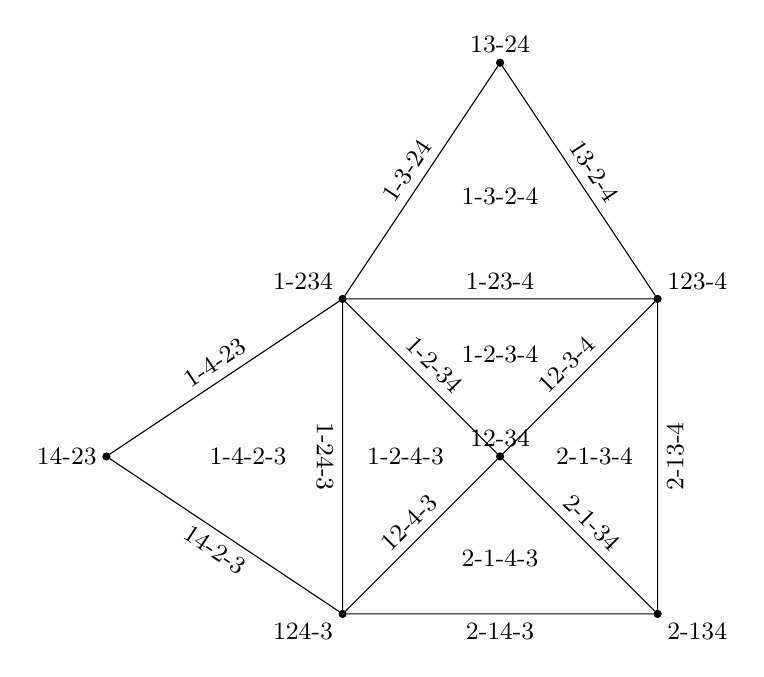
\begin{tikzpicture}

\node[draw, fill=black, circle, inner sep = 0.9pt] (u) at (0, 5) {};
\node[draw, fill=black, circle, inner sep = 0.9pt] (ul) at (-2,2) {};
\node[draw, fill=black, circle, inner sep = 0.9pt] (ur) at (2,2) {};
\node[draw, fill=black, circle, inner sep = 0.9pt] (m) at (0,0) {};
\node[draw, fill=black, circle, inner sep = 0.9pt] (bl) at (-2,-2) {};
\node[draw, fill=black, circle, inner sep = 0.9pt] (br) at (2,-2) {};
\node[draw, fill=black, circle, inner sep = 0.9pt] (l) at (-5,0) {};

\draw[-]
(ul) to node [sloped,above] {\small 1-4-23}
(l) to node [sloped,below] {\small 14-2-3}
(bl) to node [sloped,below] {\small 2-14-3}
(br) to node [sloped,below] {\small 2-13-4}
(ur) to node [sloped,above] {\small 13-2-4}
(u) to node [sloped,above] {\small 1-3-24}
(ul) to node [sloped,below] {\small 1-24-3}
(bl) to node [sloped,above] {\small 12-4-3}
(m) to node [sloped,above] {\small 12-3-4}
(ur) to node [sloped,above] {\small 1-23-4}
(ul) to node [sloped,above] {\small 1-2-34}
(m) to node [sloped,above] {\small 2-1-34}
(br);

\draw (u) node [above] {\small 13-24};
\draw (ul) node [above left] {\small 1-234};
\draw (l) node [left] {\small 14-23};
\draw (bl) node [below left] {\small 124-3};
\draw (br) node [below right] {\small 2-134};
\draw (ur) node [above right] {\small 123-4};
\draw (m) node [above] {\small 12-34};

\node at (0, 1.3) {\small 1-2-3-4};
\node at (-1.2,0) {\small 1-2-4-3};
\node at (1.2,0) {\small 2-1-3-4};
\node at (0, -1.3) {\small 2-1-4-3};
\node at (-3.2,0) {\small 1-4-2-3};
\node at (0, 3.3) {\small 1-3-2-4};
\end{tikzpicture}
\end{center}
\caption{The simplicial complex $\Sigma(\lambda)$
for $\lambda = (5,1,-2,-3)$
consisting of $7$~vertices, $12$~edges and $6$~triangles.
The empty face, labeled~$1234$, is not depicted.}
\label{figure_lambda_II}
\end{figure}


Reordering the entries of the sequence $\lambda$
does not change the complex as the following lemma shows.
\begin{lemma} If $\tau\in\mathfrak{S}_n$, then
the complexes $\Sigma(\lambda)$ and
$\Sigma(\tau(\lambda))$ are isomorphic
under the bijection
$\Sigma(\lambda) \longrightarrow \Sigma(\tau(\lambda))$
defined by $\sigma \longmapsto \tau(\sigma)$.
\label{lemma_reordering}
\end{lemma}
\begin{proof}
It is enough to observe that
$\tau(\lambda)_{\tau(B)} = \lambda_{B}$
for all subsets $B \subseteq [n]$.
\end{proof}






\section{Shellings of the Coxeter complex}
\label{section_shellings_of_Coxeter_complex}


Let $\Sigma_{n}$ be the simplicial complex formed by
the boundary of the dual of the $(n-1)$-dimensional permutahedron.
This is the type $A$ Coxeter complex.
The face poset of~$\Sigma_{n}$ is the dual poset $(\Qn)^{*}$
with the order relation of the faces in $\Sigma_{n}$ by $\leq^{*}$,
the dual order.
The permutations in $\Sym_{n}$ correspond to
the facets of $\Sigma_{n}$.
We begin by showing that $\Sigma_{n}$ is a decomposable complex.

Recall that the \emph{descent set} 
for a permutation $\tau \in \Sym_{n}$
is the set $\Des(\tau) = \{d_{1} < d_{2} < \cdots < d_{k}\}$
such that
\begin{align*}
& \tau_{1} < \tau_{2} < \cdots < \tau_{d_{1}}
>
\tau_{d_{1}+1} < \tau_{d_{1}+2} < \cdots < \tau_{d_{2}}
>
\tau_{d_{2}+1}
< 
\cdots 
<
\tau_{d_{k}} \\
& >
\tau_{d_{k}+1} < \tau_{d_{k}+2} < \cdots < \tau_{n} .
\end{align*}
Define the ordered partition $R(\tau)$ to be
$$
R(\tau)
= 
(\{\tau_{1}, \tau_{2}, \ldots, \tau_{d_{1}}\},
\{\tau_{d_{1}+1}, \tau_{d_{1}+2}, \ldots, \tau_{d_{2}}\},
\ldots,
\{\tau_{d_{k}+1}, \tau_{d_{k}+2}, \ldots, \tau_{n}\}) . 
$$
Note that the blocks of $R(\tau)$ consist of the maximal ascending runs
in the permutation~$\tau$.

Define the map $f : \Sigma_{n} \longrightarrow \Sym_{n}$
by taking an ordered partition,
ordering the elements in each block in increasing order and then
recording the elements as a permutation by reading from left to right.
Observe that, for every ordered partition $\sigma$, the permutation~$f(\sigma)$
is the minimal permutation in the weak Bruhat order
such that $\sigma\leq^* f(\sigma)$, and it is also the permutation of
minimal length such that $\sigma\leq^* f(\sigma)$.

The next two results are due to Bj\"orner;
see~\cite[Theorem~2.1]{Bjorner_II}.


\begin{prop}[Bj\"orner]
The simplicial complex $\Sigma_{n}$
is decomposable, that is, it is
given by the disjoint union
\begin{equation}
     \Sigma_{n} = \bigcup_{\tau \in \Sym_{n}} [R(\tau), \tau] .
\label{equation_disjoint_union_of_weighted_complex}
\end{equation}
\label{proposition_Sigma_decomposition}
\end{prop}
\begin{proof}
Define the map $r : \Sigma_{n} \longrightarrow \Sigma_{n}$
by iterating the following procedure.
If $C_{i}$ and $C_{i+1}$ are two adjacent blocks in the ordered partition $\sigma$
such that $\max(C_{i}) < \min(C_{i+1})$ then
merge these two blocks together.
It is clear that we have the inequalities
$r(\sigma) \leq^{*} \sigma \leq^{*} f(\sigma)$.
Also we have that $f(r(\sigma)) = f(\sigma)$
and $r(f(\sigma)) = r(\sigma)$.
Furthermore for a permutation (facet) $\tau$ we have that
$R(\tau) = r(\tau)$.
Hence each ordered partition
$\sigma$ appears only in the interval $[r(f(\sigma)), f(\sigma)]$.
Thus each ordered partition~$\sigma$ appears
exactly once 
in the union~\eqref{equation_disjoint_union_of_weighted_complex},
and hence this union is disjoint.
\end{proof}


\begin{theorem}[Bj\"orner]
Any linear extension of the weak Bruhat order is
a shelling order of the simplicial complex $\Sigma_{n}$.
\label{theorem_linear_extension_of_Bruhat_order}
\end{theorem}
\begin{proof}
Fix a linear extension of the weak Bruhat order.
Denote it by $<_{e}$.
Consider a permutation~$\tau \in \Sym_{n}$.
Let $\sigma$ be an ordered partition
such that $\sigma \leq^{*} \tau$,
that is, $\sigma$ is a face of the facet~$\tau$.
Now consider the permutation $f(\sigma)$.
Note that the permutation~$f(\sigma)$ is obtained from
the permutation~$\tau$ by merging elements together
to form blocks
and then sorting the elements in each block in increasing order.
Hence in the weak Bruhat order we have
$f(\sigma) \leq \tau$.
Hence $f(\sigma)$ appears earlier in the linear extension than $\tau$,
that is, $f(\sigma) \leq_{e} \tau$.
The result follows by
Lemma~\ref{lemma_shelling_condition}.
\end{proof}


We now consider our complex $\Sigma(\lambda)$.
\begin{theorem}
Let $\lambda = (\lambda_{1}, \ldots, \lambda_{n})$ be a sequence of
$n$ real numbers
such that $\lambdasumpositive$.
Then the complex $\Sigma(\lambda)$ is shellable.
Furthermore,
the complex $\Sigma(\lambda)$ is homeomorphic to a sphere or a ball
according to
$$
\Sigma(\lambda)
\cong
\begin{cases}
\Sss^{n-2} & \text{ if } \lambda_{1}, \lambda_{2}, \ldots, \lambda_{n} > 0, \\
\Bbbb^{n-2} & \text{ otherwise. }
\end{cases}
$$
\label{theorem_lots_of_shellings}
\end{theorem}

The proof of Theorem~\ref{theorem_lots_of_shellings}
will appear directly
after the proof of Proposition~\ref{proposition_lots_of_shellings}.



\begin{prop}
Let $\lambda \in \Rrr^{n}$ be a sequence such that
$\lambdaweaklydecreasing$ and
$\lambdasumpositive$.
Then the elements $\mathcal{A}(\lambda)$
form a lower order ideal with respect to the weak Bruhat order
on the symmetric group $\Sym_{n}$.
\label{proposition_A_lambda}
\end{prop}
\begin{proof}
Assume that
we have the following cover relation in the
weak Bruhat order:
$$
\tau
= 
\tau_{1} \cdots \tau_{j} \tau_{j+1} \cdots \tau_{n}
\coveredby
\tau_{1} \cdots \tau_{j+1} \tau_{j} \cdots \tau_{n}=\tau^{\prime}, $$
where 
$\tau_{j} < \tau_{j+1}$, and suppose that $\tau^{\prime}\in\mathcal{A}(\lambda)$.
To verify that $\tau$ belongs to $\mathcal{A}(\lambda)$,
it is enough to verify that
$\sum_{i=1}^{j} \lambda_{\tau_{i}}$ is nonnegative.
Note that
$\tau_{j} < \tau_{j+1}$
implies
$\lambda_{\tau_{j}} \geq \lambda_{\tau_{j+1}}$.
So
$\sum_{i=1}^{j} \lambda_{\tau_{i}}
\geq
\lambda_{\tau_{j+1}}
+
\sum_{i=1}^{j-1} \lambda_{\tau_{i}}$
which is positive by our assumption.
Hence
$\mathcal{A}(\lambda)$ is closed under the cover relation and
hence it is a lower order ideal in the weak Bruhat order.
\end{proof}

\begin{remark}
{\rm
A similar proof also shows that $\mathcal{A}(\lambda)$ is a
lower order ideal with respect to the \emph{strong} Bruhat order.
}
\end{remark}

\begin{prop}
Let $\lambda \in \Rrr^{n}$ be a sequence such that
$\lambdaweaklydecreasing$.
Then the weighted complex $\Sigma(\lambda)$
has the decomposition
$$ \Sigma(\lambda) = \bigcup_{\tau \in \mathcal{A}(\lambda)} [R(\tau), \tau] . $$
\label{proposition_Sigma_lambda_decomposition}
\end{prop}
\begin{proof}
By Proposition~\ref{proposition_A_lambda}
the intersection $\Sigma(\lambda) \cap [R(\tau),\tau]$
is empty if $\tau$ is not in~$\mathcal{A}(\lambda)$
and otherwise is the entire interval $[R(\tau), \tau]$.
Hence the result follows from
Proposition~\ref{proposition_Sigma_decomposition}.
\end{proof}


\begin{prop}
Let $\lambda \in \Rrr^{n}$ be a sequence such that
$\lambdaweaklydecreasing$ and 
$\lambdasumpositive$.
Then the weighted complex~$\Sigma(\lambda)$
is a partial shelling of $\Sigma_{n}$
and hence~$\Sigma(\lambda)$ is shellable.
Furthermore,
the complex~$\Sigma(\lambda)$ is homeomorphic to a sphere or a ball
according to
$$
\Sigma(\lambda)
\cong
\begin{cases}
\Sss^{n-2} & \text{ if } \lambda_{n} > 0, \\
\Bbbb^{n-2} & \text{ if } \lambda_{n} \leq 0.
\end{cases}
$$
\label{proposition_lots_of_shellings}
\end{prop}
\begin{proof}
The first statement follows by combining
Theorem~\ref{theorem_linear_extension_of_Bruhat_order}
and
Propositions~\ref{proposition_A_lambda}
and~\ref{proposition_Sigma_lambda_decomposition}.
The second statement follows
from the fact that $\Sigma_{n}$ is a sphere.
The only homology facet of the complex~$\Sigma_{n}$
is the permutation $n \cdots 21$
and it only appears as a facet in
$\Sigma(\lambda)$ if $\lambda_{n} > 0$.
\end{proof}



The proof of Theorem~\ref{theorem_lots_of_shellings}
now follows directly by combining
Lemma~\ref{lemma_reordering}
and
Proposition~\ref{proposition_lots_of_shellings}.
By taking the reduced Euler characteristic
of the simplicial complex $\Sigma(\lambda)$ in
Theorem~\ref{theorem_lots_of_shellings},
we obtain the following result 
that appears in~\cite[Corollary~A.3]{Morel} :


\begin{coro}
Let $\lambda \in \Rrr^{n}$.
Then
$$
   \sum_{\sigma \in \mathcal{P}(\lambda)} (-1)^{|\sigma|} =
   \begin{cases}
   (-1)^{n}   & \text{ if  } \lambda_{1}, \lambda_{2}, \ldots, \lambda_{n} > 0,  \\
   0        & \text{ otherwise. }
   \end{cases}
$$
\end{coro}

This corollary can also be proven by a sign-reversing involution
on the set $\mathcal{P}(\lambda)$. 
Furthermore, such a sign-reversing involution could
also be made into a discrete Morse matching;
see~\cite{Forman}.
However, the discrete Morse matching would only
give the weaker topologicial result that $\Sigma(\lambda)$
is either contractible when $\lambda_{i} \leq 0$
for some index $i$
or
homotopy equivalent to a sphere when
$\lambda_{1}, \lambda_{2}, \ldots, \lambda_{n} > 0$.


\section{The lexicographic shelling}
\label{section_lexicographic_shelling}


In this section we give a second proof that the weighted complex
$\Sigma(\lambda)$ is shellable by viewing it as the order
complex of an $EL$-shellable poset.
Throughout in this section we assume that the entries of $\lambda$
are pairwise distinct. We can always perturb $\lambda$
slightly to make this condition true. This does not
change the complex $\Sigma(\lambda)$.
We also assume that $\lambdasumpositive$.



Let $P$ be a graded poset  that 
has a minimal element $\hz$ and a maximal element $\ho$
and where all maximal chains have the same length.
Let $\mathcal{C}(P)$ be the set of all cover relations of $P$,
that is,
$$ \mathcal{C}(P) = \{(x,y) \in P^{2} \:\: : \:\: x \coveredby y\} . $$
A \emph{labeling} of a poset $P$ is a map
$\kappa$ from the set of cover relations $\mathcal{C}(P)$
to a linearly ordered set.
For a saturated chain
$c = \{x_{0} \coveredby x_{1} \coveredby \cdots \coveredby x_{k}\}$
let $\kappa(c)$
denote the word of labels, that is,
$\kappa(c) = 
\kappa(x_{0},x_{1}) \kappa(x_{1},x_{2}) \cdots \kappa(x_{k-1},x_{k})$.
For a graded poset~$P$,
an \emph{$R$-labeling} is a labeling~$\kappa$
such that in each interval $[x,y]$ there is a unique chain
$c = \{x = x_{0} \coveredby x_{1} \coveredby \cdots \coveredby x_{k} = y\}$
where the word $\kappa(c)$ is rising, that is,
$\kappa(x_{0},x_{1}) \leq \kappa(x_{1},x_{2}) \leq \cdots \leq
\kappa(x_{k-1},x_{k})$.
An \emph{$EL$-labeling} is an $R$-labeling with the extra condition
that the word $\kappa(c)$
corresponding to the
unique rising chain~$c$ in the interval $[x,y]$
is also lexicographically least
among the set of
all the words arising from saturated chains in the interval.
It is
well-known that
a poset
having an $EL$-labeling
implies that the order complex $\Delta(P - \{\hz,\ho\})$
is a shellable simplicial complex; see~\cite[Section~2]{Bjorner}.



Let $B_{n}$ denote the Boolean algebra,
that is, the collection of subsets of the set $[n]$
ordered by inclusion.
Define the subposet $B(\lambda)$
by 
$$ B(\lambda) = \{ S \in B_{n} \:\: : \:\: \lambda_{S} > 0\} \cup \{\emptyset\}. $$
Note that the full set $[n]$
belongs to $B(\lambda)$ and it is the maximal element of $B(\lambda)$.

We view this definition geometrically as follows.
Identify the vertices of the $n$-dimensional cube, that is,
$\{0,1\}^{n}$ with the Boolean algebra $B_{n}$.
The subposet $B(\lambda)$ then consists of those
vertices $(x_{1}, x_{2}, \ldots, x_{n})$
that satisfy the linear inequality
$\lambda_{1} x_{1} + \lambda_{2} x_{2} + \cdots + \lambda_{n} x_{n} > 0$
as well as the zero vector.
\begin{lemma}
Let $S$ and $T$ be two subsets in the poset $B(\lambda)$
such that $T \subsetneq S$. Let $a$ be the element
in the set difference $S-T$ with the maximal $\lambda$-value.
Then the set $T \cup \{a\}$ also belongs to $B(\lambda)$.
\label{lemma_one_step}
\end{lemma}
\begin{proof}
The proof is the same as the proof of
Lemma~\ref{lemma_split}.
If $\lambda_{a} \geq 0$ then
$\lambda_{T \cup \{a\}}
=
\lambda_{T}
+
\lambda_{a}
> 0$.
If $\lambda_{a} \leq 0$ then
all the elements in $S-T$ have non-positive $\lambda$-values,
hence
$\lambda_{T \cup \{a\}} \geq \lambda_{S} > 0$.
\end{proof}

From this straightforward observation we have
the following consequences.
\begin{prop}
The poset $B(\lambda)$ is graded of rank $n$.
Furthermore, by labeling the cover relation
$T \subsetneq S$, where $|T|+1=|S|$, 
by $-\lambda_{a}$, where $a$ is the unique element in the set difference
$S-T$, we obtain an $EL$-labeling of the poset $B(\lambda)$.
\end{prop}
\begin{proof}
By repeatedly applying Lemma~\ref{lemma_one_step}
we obtain that every interval $[T,S]$ has
a saturated chain consisting of $|S|-|T|$ steps.
Thus the poset $B(\lambda)$ has cardinality
as a rank function.
Observe that the labels of any saturated chain in the interval $[T,S]$
are the negatives
of the $\lambda$-values 
of a permutation of elements in the set difference~$S-T$.
Also, the chain obtained
by repeatedly applying Lemma~\ref{lemma_one_step}
has its labels
in increasing order.
It is the only such increasing chain. Furthermore,
it is also the lexicographically least chain.
Hence the labeling is an $EL$-labeling.
\end{proof}

Finally observe that
the order complex of $B(\lambda)$,
that is,
$\Delta(B(\lambda) - \{\hz,\ho\})$,
is the complex $\Sigma(\lambda)$.
Thus we obtain that 
we can shell the facets of $\Sigma(\lambda)$
in lexicographic order.



\section{The main result}
\label{section_main_result}

Define the map
$g : \Sigma(\lambda) \longrightarrow \Sym_{n}$
by taking  an ordered partition $\sigma$,
ordering the elements in each block in decreasing order,
and then
recording the elements as a permutation by reading from left to right.
This is similar to the map $f$ defined before
Proposition~\ref{proposition_Sigma_decomposition}.
The signs of the two permutations $f(\sigma)$ and $g(\sigma)$
are related by
$$
 (-1)^{g(\sigma)} = (-1)^{\sum_{i=1}^{k} \binom{c_{i}}{2}} \cdot (-1)^{f(\sigma)} ,
$$
where $\sigma = (C_{1},C_{2}, \ldots, C_{k})$ and $c_{i} = |C_{i}|$.

Define $S(\lambda)$ to be the sum
\begin{equation}
S(\lambda)
=
\sum_{\sigma \in \Sigma(\lambda)}
(-1)^{|\sigma|} \cdot (-1)^{g(\sigma)} . 
\label{equation_S_lambda}
\end{equation}


Let $M_{n}$ be the set of all
maximal matchings
on the set $\{1,2, \ldots,n\}$.
We say that two edges $\{a,c\}$ and $\{b,d\}$ of a matching $p$
\emph{cross} if $a<b<c<d$. Let $\cross(p)$ denote the number of crossings.
Define the sign of a matching $p$ in $M_{n}$
by
$$   (-1)^{p} = (-1)^{\cross(p)} \cdot
\begin{cases}
1 & \text{ if $n$ is even,} \\
(-1)^{i-1} & \text{ if $n$ is odd,}
\end{cases}
$$
where $i$ is the unique isolated vertex if $n$ is odd.

\begin{remark}
{\rm
When $n$ is odd
there is a sign-preserving bijection
between $M_{n}$ and $M_{n+1}$
by joining the isolated vertex $i$ to the new vertex $n+1$.
}
\label{remark_add_extra_edge}
\end{remark}








Define two functions $c_{1} : \Rrr \fl \Rrr$ and
$c_{2} : \Rrr^{2} \fl \Rrr$ in the following manner:
\[c_{1}=\ungras_{\Rrr_{>0}},
\:\:\:\: \text{ and } \:\:\:\:
c_{2}(a,b)=\left\{\begin{array}{ll}1 & \mbox{ if }a,b>0, \\
2 & \mbox{ if } a > -b \geq 0, \\
0 & \mbox{ otherwise.}\end{array}\right.\]
If $e=\{i,j\}$ is an edge with $i<j$, we set
$c(e,\lambda)=c_{2}(\lambda_{i},\lambda_{j})$.

Let $m$ be the number of edges of a maximal matching,
that is, $m = \lfloor n/2 \rfloor$.
Let~$p$ be a maximal matching in $M_{n}$.
If $n$ is even, we write $p$ as the collection of
edges~$\{e_{1}, e_{2}, \ldots, e_{m}\}$.
If $n$ is odd, the matching $p$
is of the form
$\{e_{1}, e_{2}, \ldots, e_{m}\}$
together with an isolated vertex $i$.
We set
$$
c(p,\lambda)=\prod_{j=1}^{m} c(e_{j},\lambda) 
\cdot
\begin{cases}
1 & \text{if $n$ is even,} \\
c_{1}(\lambda_{i}) & \text{if $n$ is odd.}
\end{cases}
$$



Finally, let
\begin{equation}
     T(\lambda)=\sum_{p\in M_{n}} (-1)^{p} \cdot c(p,\lambda) . 
\label{equation_T_lambda}
\end{equation}


\begin{remark}
{\rm
Following~\cite{Herb}
let $\Sym_{n}^{**}$
be the set of all permutations $\tau$
in the symmetric group $\Sym_{n}$
satisfying the inequalities
$\tau_{2j-1} < \tau_{2j}$ for
$1 \leq j \leq m$
and
$\tau_{1} < \tau_{3} < \cdots < \tau_{2m-1}$.
Then there is a bijection
$\Sym_{n}^{**} \iso M_{n}$
by sending $\tau$ to the matching
$p=\{\{\tau_{1},\tau_{2}\}, \{\tau_{3},\tau_{4}\},\ldots,
\{\tau_{2m-1},\tau_{2m}\}\}$.
Note that when $n$ is odd, the isolated vertex is $\tau_{n}$.
This bijection preserves the sign, that is,
$(-1)^{\tau} = (-1)^{p}$. 
}
\label{remark_Sn**}
\end{remark}


\begin{remark}
{\rm
When $n$ is even we can express the
sum $T(\lambda)$ as the Pfaffian of a skew-symmetric matrix.
Let $A$ be the skew-symmetric matrix of order $n$
with the upper triangular entries given by
$A_{i,j}=c_2(\lambda_{i},\lambda_{j})$.
The Pfaffian of $A$ is then the sum $T(\lambda)$. (See Remark \ref{remark_Sn**}.)

Similarly, when $n$ is odd, we use the bijection in
Remark~\ref{remark_add_extra_edge}.
In this case let $A$ be the skew-symmetric
matrix of order $n+1$ where
the upper triangular entries are 
$$ A_{i,j}
=
\begin{cases}
c_{2}(\lambda_{i},\lambda_{j})
& \text{ if } 1 \leq i < j \leq n , \\
c_{1}(\lambda_{i})
& \text{ if } 1 \leq i \leq n, j=n+1 .
\end{cases}
$$
Again the Pfaffian of $A$ is the sum $T(\lambda)$.
}
\end{remark}

We can now state the main result.
This
is Proposition~A.4 of~\cite{Morel}.
